\documentclass[11pt,letter]{article}

\usepackage[latin1]{inputenc}
\usepackage{amsmath}
\usepackage{amsfonts}
\usepackage{amssymb}
\usepackage{amsthm}
\usepackage{enumitem}
\usepackage[english]{babel}
\usepackage{fancyhdr}
\usepackage{lipsum}
\usepackage{chngpage}
\usepackage{geometry}
\usepackage{mathtools}
\usepackage{tabularx}
\usepackage{verbatim}
\usepackage{enumitem}
\usepackage{tikz}
\usepackage[ruled,vlined]{algorithm2e}
\geometry{letterpaper, portrait, margin=1in}
 
\pagestyle{fancy}
\fancyhf{}
\rhead{\thepage}
\lhead{Implementing Path 3-Coloring and Path 3-Choosing Algorithms on Plane Graphs}
\rfoot{}

\newcommand{\overbar}[1]{\mkern 1.5mu\overline{\mkern-1.5mu#1\mkern-1.5mu}\mkern 1.5mu}

\begin{document}

\title{Implementing Path 3-Coloring and Path 3-Choosing Algorithms on Plane Graphs}
\author{Aven Bross}
\date{August 26, 2016}

\maketitle

\section*{Abstract}

Path coloring a graph partitions its vertices into sets inducing a disjoint union of paths. In this project
we consider several algorithms to compute path colorings of graphs embedded in the plane. We
first implement an algorithm to path 3-color plane graphs from Poh's proof in [4]. Second, we present a linear time
implementation of an algorithm to path 3-choose plane graphs from the independant work of Hartman [1] and
Skrekovski [2].

\section{Introduction}

All graphs discussed in this project will be simple, undirected, and finite. We say a graph is planar if it may
be drawn in the plane without edge crossings, known as a plane drawing. A planar embedding of a graph is an
ordering of the edges around each vertex according to a plane drawing. A plane graph is a graph with a
planar embedding.
A $k$-coloring of a graph partitions its vertices into $k$ color classes. Such a coloring is called proper
if each color class consists of snonadjacent vertices.\\

\noindent Appel and Haken [d,e] display that all planar graphs have a proper $4$-coloring.
This result is best possible and known as the Four Color Theorem.
Generalizations of proper coloring were introduced in [f,g,h] allowing color classes to form forests, or allowing
vertices share a color with some bounded number of neighbors. Cowen et al. ([j]) show all planar
graphs may be $3$-colored such that each vertex shares a color with at most two neighbors.\\

\noindent We will be considering the problem of path coloring, producing a $k$-coloring of a graph such that each color
class induces a disjoint union of paths. A disjoint union of paths is equivalent to a linear forest, a forest
where each component is a path. This coloring
was introduced by Harary in [i]. Note that this is similar to the defective coloring of Cowen et al. above,
with the added restriction that path coloring forbids cycles. In [4] Poh displayes that all
planar graphs have a path $3$-coloring. We present an implementation of Poh's algorithm to path
$3$-color plane graphs.\\

\noindent Given a list of $k$ colors for each vertex, a $k$-list-coloring, or $k$-choosing, assigns each vertex a
color from its list.
If a graph has a proper $k$-choosing it is said to be $k$-choosable. List-coloring was first introduced by
Erd{\"o}s et al. in [m]. Thomassen in [5] proves that all planar graphs are $5$-choosable. Planar
graphs that are not $4$-choosable are described by Mirzakhani in [o] and Voigt in [p], so Thomassen's result
is best possible. Jensen and Toft in [t] note that Thomassen's proof yields a linear algorithm for $5$-choosing
plane graphs.\\

\noindent Hull and Eaton in [3] prove planar graphs are $3$-choosable such that each vertex shares a color with
at most two neighbors, and furthermore show this result is best possible. Hartman in [1] and Skrekovski in [2]
independantly provide similar proofs that planar graphs are path $3$-choosable. Hartman claims the proof yields
a linear time algorithm for path $3$-list-coloring, and thus path $3$-coloring, plane graphs. We present a
linear time implementation of Hartman and Skrekovski's algorithm.

\section{Path $3$-Coloring Plane Graphs}

We first restate the theorem and proof of Poh [4]. This proof yields a simple algorithm for path $3$-coloring
plane graphs.\\

\begin{adjustwidth}{1.5em}{1.5em}
\noindent\textbf{Theorem 1.} Let $G$ be a $2$-connected weakly triangulated plane graph or a complete
graph on two vertices and
suppose the outer face $C$ has been $2$-colored such that each color class induces a non-empty path. This
$2$-coloring may be extended to a path $3$-coloring of $G$ such that no vertex in $V(C)$ recieves a same color
neighbor in $V(G)\setminus V(C)$.\\
\end{adjustwidth}

\begin{proof}
\noindent If $|V(G)|\le 3$ the coloring follows trivially. Let $|V(G)|>3$ and suppose the theorem holds
for all graphs $H$ with $|V(H)|<|V(G)|$. Let $P=p_0\ldots p_n$ and $Q=q_0\ldots q_m$ denote the two induced paths from the $2$-coloring of $C$
such that the edges $p_0q_0$ and $p_nq_m$ are in $C$. Suppose there exist uncolored vertices, that is
$V(G)\setminus V(C)\ne\emptyset$.\\

\noindent Let $t_0$ be the vertex forming a face with $p_0$ and $q_0$. If $t_0\in P$, this face is already
colored and we consider the graph bounded by $P-p_0$ and $Q$. Similarly, if $t_0\in Q$ then the inductive
hypothesis applies to the graph bounded by $P$ and $Q-q_0$. Let $t_1$ be the vertex forming a face with $p_n$
and $q_m$ and proceed in the same manner until $t_1$ is not in either path.\\

\noindent Suppose there exists an induced path $T$ from $t_0$ to $t_1$. We color $T$ the remaining color not
assigned to $P$ or $Q$ and apply the inductive hypothesis to the subgraph bounded by $P$ and $T$, and the
subgraph bounded by $T$ and $Q$. With only the path $T$ in common between the two subgraphs, the combined
$3$-coloring forms a path coloring of $G$.\\

\noindent Suppose no such path exists from $t_0$ to $t_1$. Since $G$ is weakly triangulated there must exist an
edge $p_iq_j\in E(G)\setminus E(C)$ with $p_i\in P$ and $q_j\in Q$. We separately apply the inductive hypothesis
to the subgraph bounded by $p_0\ldots p_i$ and $q_0\ldots q_j$, and the subgraph bounded by $p_i\ldots p_n$ and
$q_j\ldots q_m$. The two subgraphs only share the vertices $p_i$ and $q_j$, thus the combined $3$-coloring forms
a path coloring of $G$.\\
\end{proof}

\begin{adjustwidth}{1.5em}{1.5em}
\noindent\textbf{Corollary 2.} All plane graphs are path $3$-colorable.\\
\end{adjustwidth}

\begin{proof}
Let $G$ be a plane graph. Since adding edges does not make $G$ easier to color, augment $G$ with edges until
it is triangulated. Path $2$-color the outer triangle and apply Theorem 1 to path $3$-color $G$.\\
\end{proof}

\subsection*{Poh's Algorithm}

\noindent Let $G$ be a weakly triangulated plane graph with outer face formed by the two monocolor paths $P$ and
$Q$, each colored sdistinct color. Poh's path $3$-coloring algorithm proceeds as follows:

\begin{enumerate}
\item If all vertices in $G$ are colored, terminate;
\item Locate the vertex $t_1$. If $t_1\in P$ remove $p_n$ and repeat. If $t_1\in Q$ remove $q_m$ and
repeat;

\begin{center}
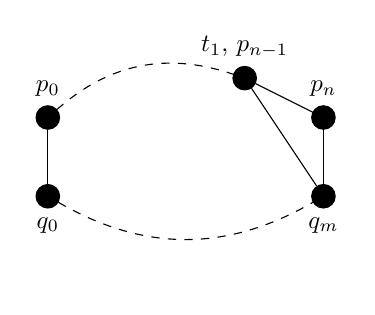
\begin{tikzpicture}[
		scale=1,
		every node/.style={circle, draw, minimum size=1mm, scale=0.9},
		every label/.append style={rectangle}
	]
  \node (p0) [label=above:$p_0$, fill] at (-1.5cm, 0.5cm) {};
  \node (pn) [label=above:$p_n$, fill] at (2cm, 0.5cm) {};
  \node (q0) [label=below:$q_0$, fill] at (-1.5cm, -0.5cm) {};
  \node (qn) [label=below:$q_m$, fill] at (2cm, -0.5cm) {};
  \node (t) [label=above:{$t_1$, $p_{n-1}$}, fill] at (1cm, 1cm) {};
  \node (null) [draw=none] at (270:1.5cm) {};
  
  \draw (t) edge (pn);
  \draw (qn) edge (t);
  \draw (p0) edge [bend left] (t) [dashed];
  \draw (q0) edge [bend right] (qn) [dashed];
  \draw (p0) edge (q0);
  \draw (pn) edge (qn);
\end{tikzpicture}
$\qquad$
\begin{tikzpicture}[
		scale=1,
		every node/.style={circle, draw, minimum size=1mm, scale=0.9},
		every label/.append style={rectangle}
	]
  \node (null) [draw=none] at (0cm, 0cm) {$\rightarrow$};
  \node (null) [draw=none] at (270:1.5cm) {};
\end{tikzpicture}
$\qquad$
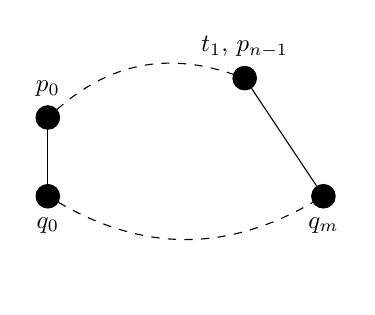
\begin{tikzpicture}[
		scale=1,
		every node/.style={circle, draw, minimum size=1mm, scale=0.9},
		every label/.append style={rectangle}
	]
  \node (p0) [label=above:$p_0$, fill] at (-1.5cm, 0.5cm) {};
  \node (q0) [label=below:$q_0$, fill] at (-1.5cm, -0.5cm) {};
  \node (qn) [label=below:$q_m$, fill] at (2cm, -0.5cm) {};
  \node (t) [label=above:{$t_1$, $p_{n-1}$}, fill] at (1cm, 1cm) {};
  \node (null) [draw=none] at (270:1.5cm) {};
  
  \draw (qn) edge (t);
  \draw (p0) edge [bend left] (t) [dashed];
  \draw (q0) edge [bend right] (qn) [dashed];
  \draw (p0) edge (q0);
\end{tikzpicture}
\hfill\\

\textbf{Figure 2.1} The case $t_1\in P$.
\end{center}

\item Perform a breadth first search from $t_1$;
\item Terminate the search when we find a vertex $u$ with adjacent neighbors $p_i$ and $q_j$;
\item Color with the remaining color the induced $ut_1$-path determined by the breadth first search;
\item Apply the algorithm to the subgraph bounded by the $p_0p_i$-path and $q_0q_i$-path, the subgraph
bounded by the $p_ip_n$-path and $ut_1$-path, and the subgraph bounded by the $ut_1$-path and $q_jq_m$-path.
\end{enumerate}

\begin{center}
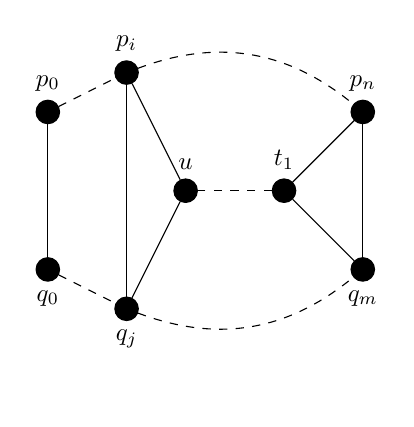
\begin{tikzpicture}[
		scale=1,
		every node/.style={circle, draw, minimum size=1mm, scale=0.9},
		every label/.append style={rectangle}
	]
  \node (p0) [label=above:$p_0$, fill] at (-2cm, 1cm) {};
  \node (pn) [label=above:$p_n$, fill] at (2cm, 1cm) {};
  \node (q0) [label=below:$q_0$, fill] at (-2cm, -1cm) {};
  \node (qn) [label=below:$q_m$, fill] at (2cm, -1cm) {};
  \node (t0) [label=above:$u$, fill] at (-0.25cm, 0cm) {};
  \node (t1) [label=above:$t_1$, fill] at (1cm, 0cm) {};
  \node (pi) [label=above:$p_i$, fill] at (-1cm, 1.5cm) {};
  \node (qj) [label=below:$q_j$, fill] at (-1cm, -1.5cm) {};
  \node (null) [draw=none] at (270:2.5cm) {};
  \draw (p0) edge (pi) [dashed];
  \draw (pi) edge [bend left] (pn) [dashed];
  \draw (q0) edge (qj) [dashed];
  \draw (qj) edge [bend right] (qn) [dashed];
  \draw (p0) edge (q0);
  \draw (pn) edge (qn);
  \draw (pi) edge (qj);
  \draw (pn) edge (t1);
  \draw (qn) edge (t1);

  \draw (t1) edge (t0) [dashed];
  \draw (pi) edge (t0);
  \draw (qj) edge (t0);
\end{tikzpicture}
$\qquad$
\begin{tikzpicture}[
		scale=1,
		every node/.style={circle, draw, minimum size=1mm, scale=0.9},
		every label/.append style={rectangle}
	]
  \node (null) [draw=none] at (0cm, 0cm) {$\rightarrow$};
  \node (null) [draw=none] at (270:2.5cm) {};
\end{tikzpicture}
$\qquad$
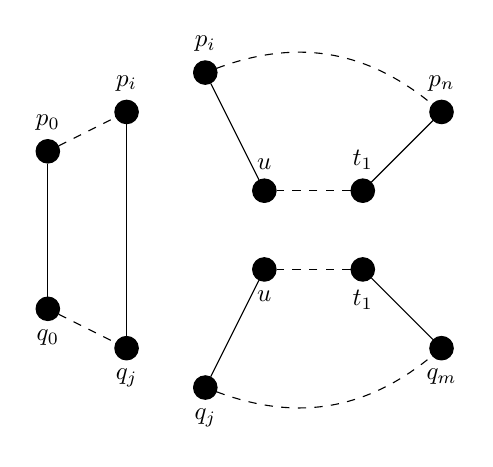
\begin{tikzpicture}[
		scale=1,
		every node/.style={circle, draw, minimum size=1mm, scale=0.9},
		every label/.append style={rectangle}
	]
  \node (p0) [label=above:$p_0$, fill] at (-3cm, 1cm) {};
  \node (q0) [label=below:$q_0$, fill] at (-3cm, -1cm) {};
  \node (pi) [label=above:$p_i$, fill] at (-2cm, 1.5cm) {};
  \node (qj) [label=below:$q_j$, fill] at (-2cm, -1.5cm) {};
  
  \node (pi_1) [label=above:$p_i$, fill] at (-1cm, 2cm) {};
  \node (pn) [label=above:$p_n$, fill] at (2cm, 1.5cm) {};
  \node (t0) [label=above:$u$, fill] at (-0.25cm, 0.5cm) {};
  \node (t1) [label=above:$t_1$, fill] at (1cm, 0.5cm) {};
  
  \node (qj_1) [label=below:$q_j$, fill] at (-1cm, -2cm) {};
  \node (qn) [label=below:$q_m$, fill] at (2cm, -1.5cm) {};
  \node (t0_1) [label=below:$u$, fill] at (-0.25cm, -0.5cm) {};
  \node (t1_1) [label=below:$t_1$, fill] at (1cm, -0.5cm) {};
  \node (null) [draw=none] at (270:2.5cm) {};
  \draw (p0) edge (pi) [dashed];
  \draw (pi_1) edge [bend left] (pn) [dashed];
  \draw (q0) edge (qj) [dashed];
  \draw (qj_1) edge [bend right] (qn) [dashed];
  \draw (p0) edge (q0);
  \draw (pi) edge (qj);
  \draw (pn) edge (t1);
  \draw (qn) edge (t1_1);
  \draw (t1) edge (t0) [dashed];
  \draw (t1_1) edge (t0_1) [dashed];
  \draw (pi_1) edge (t0);
  \draw (qj_1) edge (t0_1);
\end{tikzpicture}
\hfill\\
\textbf{Figure 2.2} Dividing $G$ along the edge $p_iq_j$ and the $ut_1$-path.
\end{center}

\subsection*{Implementing Poh's Algorithm}

Let the plane graph $G$ be represented as an incidence list (or adjacency list) and an ordering of edges (neighbors) around
each vertex following a
combinatorial embedding. We track the paths $P$ and $Q$ by marking each vertex with its respective path and
storing the path start and end vertices $p_0$, $p_n$, $q_0$, and $q_m$.
We first find $t_1$ by looking through the ordered neighbors of $q_m$ and take the vertex counterclockwise past
$p_n$. This step is repeated until the graph is colored or $t_1\not\in P\cup Q$.\\

\noindent We perform a
breadth first search starting at $t_1$ and storing parents for each vertex visited. Vertices marked to be in $P$
or $Q$ will be ignored, in this way containing the search within the current bounded subgraph. The
search terminates once a vertex $u$ with adjacent neighbors $p_i\in P$ and $q_j\in Q$ has been reached. An
induced $ut_1$-path is produced by backtracking through the search from $u$. We color and mark each vertex on the
new path with the remaining color not used to color $P$ or $Q$.\\

\noindent To color the remaining graph we recurse on both the region
bounded by the $p_ip_n$-path and $ut_1$-path, and the region bounded by the $ut_1$-path and $q_jp_m$-path.
If $p_i=p_0$ and $q_j=q_0$ we are done and this mimicks the case of a $t_0t_1$ path in with $u=t_0$.
If $p_i\ne p_0$ or $q_j\ne q_0$ we handle the remaining subgraph by recursing on the region bounded by the
$p_0p_i$-path and $q_0p_j$-path. Note each recursive step is independant and vertex marks are shared so the
algorithm may instead proceed iteratively by pushing paths, represented by their start and end
vertices, into a stack or queue.

\subsection*{Time Complexity}

\noindent Locating $t_1$ requires a single neighbor lookup. The average complexity of a neighbor lookup is
$O(|E|/|V|)$. Each vertex may be $t_1$ at most once so over the entire graph we perform at most $|V|$ neighbor
lookups. In planar graphs $|E|\le 3|V|-6$, and $O(|E|)=O(|V|)$. Therefore, the
complexity of this step is $O(|V|^2/|V|)=O(|V|)$. We also perform at most one breadth first
search from each $t_1$ with complexity $O(|V|)$. Therefore the complexity of the serach step over the
entire graph is $O(|V|^2)$. This gives an overall complexity of $O(|V|+|V|^2)=O(|V|^2)$.

\section{Path $3$-Choosing Plane Graphs}

The following is a restatment of a theorem of Hartman [1] and Skrekovski [2]. We provide a slight modification of
the proof technique that wraps the path coloring and path removal portions of Hartman's proof into a single inductive
step that considers only the last vertex colored on the current path, which will be denoted $p$.
This modification is motivated by the relative simplicity of removing a single outer face vertex,
compared with removing an entire path.
We will show this proof yields a linear time algorithm and implementation, as claimed by Hartman in [1].\\

\noindent The informal idea followed in both the proof and algorithm is to start with
vertices $x$ and $y$ on the outer face and draw a path clockwise between them using vertices on the outer face.
We mark the current color of the path with $\alpha$ and the current end of the path with $p$. At each step we will remove
$p$ and look for a vertex between $p$ and $y$ on the outer face to color $\alpha$ and extend our path. If no
such vertex is found, or we reach and remove $y$, we move $p$ back to $x$ and start a new path.\\

\noindent To avoid dealing with disconnected graphs the algorithm will separately consider the $2$-connected
components produced when removing
$p$ results in cutvertices. In fact, we incrementally remove $p$ and halt once a single cutvertex is found.
The algorithm then
considers the two maximal $2$-connected components separately. We will continue to remove $p$ from the component
it is contained in.\\

\noindent Suppose $C$ is
the outer cycle of a $2$-connected weakly triangulated plane graph $G$. Using notation from [1] for $u,v\in V(C)$
we let $C[u,v]$ denote the path from $u$ to $v$ clockwise along the outer face. If we wish to exclude $u$ or $v$
from this path we will use parenthesis, $C(u,v)$. Similarly, for $v\in V(G)$ and
$u,w\in N(v)$ we let $[u,w]_v$ denote the path from $u$ to $w$ clockwise around $v$, assuming triangulated
faces.\\

\noindent Note that in all figures solid circles denote vertices yet to be colored, and colored vertices will
be labeled with their assigned color. We have $\alpha$ denote the current path color and a label $\beta$ represent
coloring $v$ from $L(v)\setminus\{\alpha\}$. If a vertex $v$ is unlabled it represents arbitrary coloring from
$L(v)$.\\

\begin{adjustwidth}{1.5em}{1.5em}
\noindent\textbf{Theorem 3.} Let $G$ be a $2$-connected weakly triangulated plane graph, or a complete graph
on one or two vertics, with outer face $C$. 
Let $x,y\in V(C)$ be not necessarily distinct, potentially precolored vertices. Let $p\in C[x,y]$ be precolored some
color $\alpha$. Suppose $L(v)$ assigns a list of colors to each $v\in V(G)$ that has not been precolored such that
\[
    \begin{array}{ll}
	    |L(v)|\ge 1 & \text{if } v=x \text{ or } v=y;\\
	    |L(v)|\ge 2 & \text{if } v\in V(C)\setminus\{x,y\};\\
	    |L(v)|\ge 3 & \text{otherwise.}
    \end{array}
\]
If $p\ne x$, let $\alpha\not\in L(v)$ for
any $v\in V(C[x,p))$. Also assume the precoloring is a path coloring.\\

\noindent The coloring may be extended to
a path choosing of $G$ from $L$ such that $x$, $y$, and $p$ each share a color with at most one neighbor. If
$x=y$ then $x$ and $y$ each share a color with none of their neighbors. If $y=p$, or $y$ is immediately prior to
$p$ on the outer face and $\alpha\not\in L(y)$, then $y$ shares a color with none of its neighbors.\\
\end{adjustwidth}

\begin{proof}
If $|V(G)\le 2$ the theorem easily follows. Suppose $|V(G)|>2$ and the theorem
holds for all graphs $H$ with $|V(H)|<|V(G)|$. Let
$C=c_0c_1\ldots c_n$ denote, in clockwise order, the outer face of $G$ with $p=c_0$.
There are several cases to consider. Let $c_i$ be the next vertex in $V(C)\cap N(p)$ counterclockwise from $c_n$.
Let $G_0$ be the subgraph bounded by the cycle formed from $C[2_i,c_n]$ and $[2_n,c_i]_p$. If $c_i\ne c_1$ let
$G_1$ be the sugbraph bounded by the cycle formed from $C[p,c_i]$ and the edge $pc_i$. As seen in Figure
3.1 $G=G_0\cup G_1$ and $V(G_0)\cap V(G_1)=\{c_i\}$.
We will display in each case that the inductive hypothesis holds for each subgraph and their union still
forms a path choosing of $G$ from $L$.
If $c_i=c_1$ we will say $G_1$ does not exist and handle this case specially, noting $G_0=G-p$.

\begin{center}
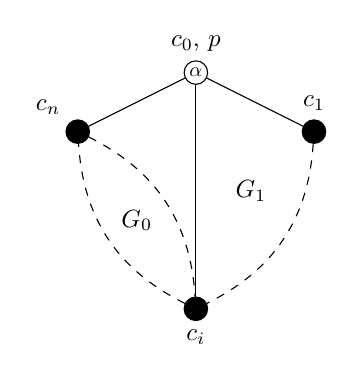
\begin{tikzpicture}[
		scale=1,
		every node/.style={circle, draw, minimum size=1mm, scale=0.9},
		every label/.append style={rectangle}
	]
  \node (c_n) [label=above left:$c_n$, fill] at (-1.5cm, 1.25cm) {};
  \node (p) [label=above:{$c_0$, $p$}] at (0cm, 2cm) {};
  \node (p_label) [draw=none, scale=0.8] at (0cm, 2cm) {$\alpha$};
  \node (c_1) [label=above:$c_1$, fill] at (1.5cm, 1.25cm) {};
  \node (c_i) [label=below:$c_i$, fill] at (0cm, -1cm) {};
  \node (G_0) [draw=none, ] at (-0.75cm, 0.12cm) {$G_0$};
  \node (G_1) [draw=none] at (0.7cm, 0.5cm) {$G_1$};
  \node (null) [draw=none] at (270:1.5cm) {};
  \draw (c_i) edge [bend left] (c_n) [dashed];
  \draw (c_n) edge [bend left] (c_i) [dashed];
  \draw (c_n) edge (p);
  \draw (p) edge (c_1);
  \draw (p) edge (c_i);
  \draw (c_1) edge [bend left] (c_i) [dashed];
\end{tikzpicture}
\hfill\\
\textbf{Figure 3.1} The subdivision of $G$ into $G_0$ and $G_1$.
\end{center}

\noindent For all $v\in (N(p)\cap V(G_0))\setminus\{x,y\}$ we note if $v=c_n$ or $v=c_i$
then $|L(v)|\ge 2$, and $|L(v)|\ge3$ otherwise. We define a new list assignment $L_0$
such that $L_0(v)=L(v)\setminus\{\alpha\}$ for
$v\in N(p)\cap V(G_0)$, and $L_0(v)=L(v)$ for $v\in V(G_0)\setminus N(p)$. Note that all
$v\in N(p)\cap V(G_0)$ will be on the outer face of $G_0$. Thus $|L_0(v)|\ge 3$ for all interior
vertices $v$ of $G_0$. Except for a few special cases for $y$ mentioned below, $|L_0(v)|\ge 1$ for all
$v\in\{x,y,c_i,c_n\}$. Finally, $|L_0(v)|\ge2$ for all other $v$ on the outer face of $G_0$. By choosing $G_0$ from
$L_0$ we ensure either $p$ recieves no $\alpha$ colored neighbors in $G_0$ unless $c_i$ is colored $\alpha$.
If $c_i$ is colored $\alpha$ then $p$ recieves no $\alpha$ colored neighbors in $G_1$ other than $c_i$.

\begin{center}
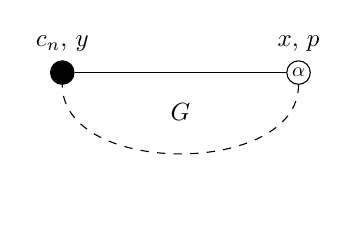
\begin{tikzpicture}[
		scale=1,
		every node/.style={circle, draw, minimum size=1mm, scale=0.9},
		every label/.append style={rectangle}
	]
  \node (c_n) [label=above:{$c_n$, $y$}, fill] at (-1.5cm, 0cm) {};
  \node (p) [label=above:{$x$, $p$}] at (1.5cm, 0cm) {};
  \node (p_label) [draw=none, scale=0.8] at (1.5cm, 0cm) {$\alpha$};
  \node (G) [draw=none, ] at (0cm, -0.5cm) {$G$};
  \node (null) [draw=none] at (270:1.5cm) {};
  \draw (p) edge [bend left=90] (c_n) [dashed];
  \draw (c_n) edge (p);
\end{tikzpicture}
$\quad$
\begin{tikzpicture}[
		scale=1,
		every node/.style={circle, draw, minimum size=1mm, scale=0.9},
		every label/.append style={rectangle}
	]
  \node (null) [draw=none] at (0cm, -0.5cm) {$\rightarrow$};
  \node (null) [draw=none] at (270:1.5cm) {};
\end{tikzpicture}
$\quad$
\begin{tikzpicture}[
		scale=1,
		every node/.style={circle, draw, minimum size=1mm, scale=0.9},
		every label/.append style={rectangle}
	]
  \node (c_n) [label=above:{$x'$, $p'$}] at (-1.5cm, 0cm) {};
  \node (c_n_label) [draw=none, scale=0.8] at (-1.5cm, 0cm) {$\alpha$};
  \node (p) [label=above:{$y'$}] at (1.5cm, 0cm) {};
  \node (p_label) [draw=none, scale=0.8] at (1.5cm, 0cm) {$\alpha$};
  \node (G) [draw=none, ] at (0cm, -0.5cm) {$G$};
  \node (null) [draw=none] at (270:1.5cm) {};
  \draw (p) edge [bend left=90] (c_n) [dashed];
  \draw (c_n) edge (p);
\end{tikzpicture}
\hfill\\
\textbf{Figure 3.2} The case $x=p$, $y=c_n$, and $\alpha\in L(y)$.
\end{center}

\noindent If $\alpha\in L(y)$ and $y\in V(G_0)\cap N(p)$ it may be that $|L_0(y)|=0$. Note that in the case $y$
has been precolored a color distinct from $\alpha$ we will say $\alpha\not\in L(v)$. To handle this we
first note $y\in\{c_n, c_i\}$. The case $y=c_i$ will require no special treatment as $c_i$ will
naturally be colored $\alpha$. Suppose $\alpha\in L(y)$ and $y=c_n$. Then $x=p$, since otherwise $y\in C[x,p)$ and
$\alpha\not\in L(y)$. Color $y$ with $\alpha$ and apply the inductive hypothesis to choose
$G$ from $L$ with $x'=y$, $y'=x$, and $p'=y$. Otherwise suppose if $\alpha\in L(y)$ then $y\ne c_n$.

\begin{center}
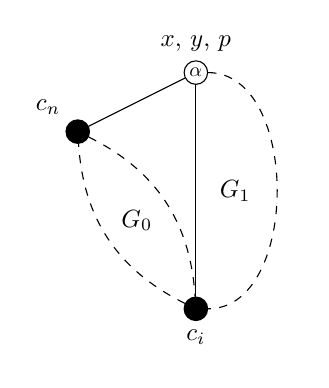
\begin{tikzpicture}[
		scale=1,
		every node/.style={circle, draw, minimum size=1mm, scale=0.9},
		every label/.append style={rectangle}
	]
  \node (c_n) [label=above left:$c_n$, fill] at (-1.5cm, 1.25cm) {};
  \node (p) [label=above:{$x$, $y$, $p$}] at (0cm, 2cm) {};
  \node (p_label) [draw=none, scale=0.8] at (0cm, 2cm) {$\alpha$};
  \node (c_i) [label=below:$c_i$, fill] at (0cm, -1cm) {};
  \node (G_0) [draw=none, ] at (-0.75cm, 0.12cm) {$G_0$};
  \node (G_1) [draw=none] at (0.5cm, 0.5cm) {$G_1$};
  \node (null) [draw=none] at (270:1.5cm) {};
  \draw (c_i) edge [bend left] (c_n) [dashed];
  \draw (c_n) edge [bend left] (c_i) [dashed];
  \draw (c_n) edge (p);
  \draw (p) edge (c_i);
  \draw (p) edge [bend left=90] (c_i) [dashed];
\end{tikzpicture}
$\quad$
\begin{tikzpicture}[
		scale=1,
		every node/.style={circle, draw, minimum size=1mm, scale=0.9},
		every label/.append style={rectangle}
	]
  \node (null) [draw=none] at (0cm, 0.5cm) {$\rightarrow$};
  \node (null) [draw=none] at (270:1.5cm) {};
\end{tikzpicture}
$\quad$
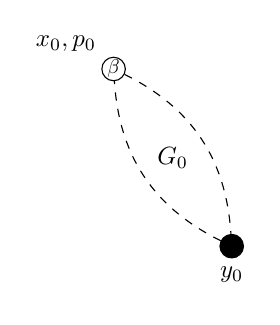
\begin{tikzpicture}[
		scale=1,
		every node/.style={circle, draw, minimum size=1mm, scale=0.9},
		every label/.append style={rectangle}
	]
  \node (c_n) [label=above left:{$x_0,p_0$}] at (-1.5cm, 1.25cm) {};
  \node (c_i) [label=below:$y_0$, fill] at (0cm, -1cm) {};
  \node (c_n_label) [draw=none, scale=0.8] at (-1.5cm, 1.25cm) {$\beta$};
  \node (G_0) [draw=none] at (-0.75cm, 0.12cm) {$G_0$};
  \node (null) [draw=none] at (270:1.5cm) {};
  \draw (c_i) edge [bend left] (c_n) [dashed];
  \draw (c_n) edge [bend left] (c_i) [dashed];
\end{tikzpicture}
$\quad$
\begin{tikzpicture}[
		scale=1,
		every node/.style={circle, draw, minimum size=1mm, scale=0.9},
		every label/.append style={rectangle}
	]
  \node (null) [draw=none] at (0cm, 0.5cm) {$\rightarrow$};
  \node (null) [draw=none] at (270:1.5cm) {};
\end{tikzpicture}
$\quad$
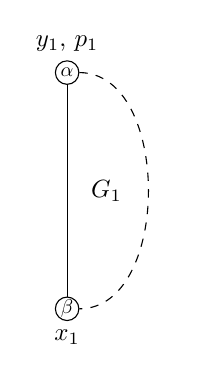
\begin{tikzpicture}[
		scale=1,
		every node/.style={circle, draw, minimum size=1mm, scale=0.9},
		every label/.append style={rectangle}
	]
  \node (p) [label=above:{$y_1$, $p_1$}] at (0cm, 2cm) {};
  \node (p_label) [draw=none, scale=0.8] at (0cm, 2cm) {$\alpha$};
  \node (c_i) [label=below:$x_1$] at (0cm, -1cm) {};
  \node (c_i_label) [draw=none, scale=0.8] at (0cm, -1cm) {$\beta$};
  \node (G_1) [draw=none] at (0.5cm, 0.5cm) {$G_1$};
  \node (null) [draw=none] at (270:1.5cm) {};
  \draw (p) edge (c_i);
  \draw (p) edge [bend left=90] (c_i) [dashed];
\end{tikzpicture}
\hfill\\
\textbf{Figure 3.3} The case $x=y=p$.
\end{center}

\noindent Suppose $x=y=p$. Color $c_i$ from $L_0(c_i)$. Apply the inductive hypothesis to choose $G_0$ from
$L$ with $x_0=c_n$, $y_0=p_0=c_i$. If $G_1$ exists we apply the inductive hypothesis again to choose $G_1$ from
$L$ with $x_1=c_i$, $y_1=y$, and $p_1=p$. Since $c_i$ recieves at most one neighbor in each $G_0$ and $G_1$, the
combined coloring forms a path choosing of $G$ from $L$.

\begin{center}
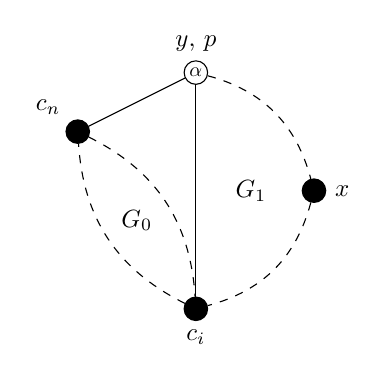
\begin{tikzpicture}[
		scale=1,
		every node/.style={circle, draw, minimum size=1mm, scale=0.9},
		every label/.append style={rectangle}
	]
  \node (c_n) [label=above left:$c_n$, fill] at (-1.5cm, 1.25cm) {};
  \node (p) [label=above:{$y$, $p$}] at (0cm, 2cm) {};
  \node (p_label) [draw=none, scale=0.8] at (0cm, 2cm) {$\alpha$};
  \node (x) [label=right:$x$, fill] at (1.5cm, 0.5cm) {};
  \node (c_i) [label=below:$c_i$, fill] at (0cm, -1cm) {};
  \node (G_0) [draw=none] at (-0.75cm, 0.12cm) {$G_0$};
  \node (G_1) [draw=none] at (0.7cm, 0.5cm) {$G_1$};
  \node (null) [draw=none] at (270:1.5cm) {};
  \draw (c_i) edge [bend left] (c_n) [dashed];
  \draw (c_n) edge [bend left] (c_i) [dashed];
  \draw (c_n) edge (p);
  \draw (p) edge (c_i);
  \draw (p) edge [bend left] (x) [dashed];
  \draw (x) edge [bend left] (c_i) [dashed];
\end{tikzpicture}
$\quad$
\begin{tikzpicture}[
		scale=1,
		every node/.style={circle, draw, minimum size=1mm, scale=0.9},
		every label/.append style={rectangle}
	]
  \node (null) [draw=none] at (0cm, 0.5cm) {$\rightarrow$};
  \node (null) [draw=none] at (270:1.5cm) {};
\end{tikzpicture}
$\quad$
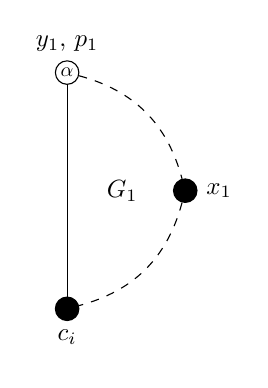
\begin{tikzpicture}[
		scale=1,
		every node/.style={circle, draw, minimum size=1mm, scale=0.9},
		every label/.append style={rectangle}
	]
  \node (p) [label=above:{$y_1$, $p_1$}] at (0cm, 2cm) {};
  \node (p_label) [draw=none, scale=0.8] at (0cm, 2cm) {$\alpha$};
  \node (x) [label=right:$x_1$, fill] at (1.5cm, 0.5cm) {};
  \node (c_i) [label=below:$c_i$,fill] at (0cm, -1cm) {};
  \node (G_1) [draw=none] at (0.7cm, 0.5cm) {$G_1$};
  \node (null) [draw=none] at (270:1.5cm) {};
  \draw (p) edge (c_i);
  \draw (p) edge [bend left] (x) [dashed];
  \draw (x) edge [bend left] (c_i) [dashed];
\end{tikzpicture}
$\quad$
\begin{tikzpicture}[
		scale=1,
		every node/.style={circle, draw, minimum size=1mm, scale=0.9},
		every label/.append style={rectangle}
	]
  \node (null) [draw=none] at (0cm, 0.5cm) {$\rightarrow$};
  \node (null) [draw=none] at (270:1.5cm) {};
\end{tikzpicture}
$\quad$
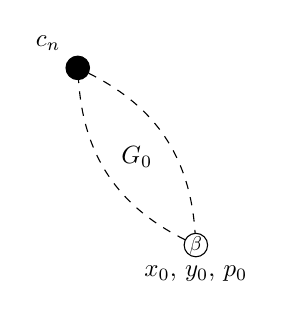
\begin{tikzpicture}[
		scale=1,
		every node/.style={circle, draw, minimum size=1mm, scale=0.9},
		every label/.append style={rectangle}
	]
  \node (c_n) [label=above left:{$c_n$}, fill] at (-1.5cm, 1.25cm) {};
  \node (c_i) [label=below:{$x_0$, $y_0$, $p_0$}] at (0cm, -1cm) {};
  \node (c_i_label) [draw=none, scale=0.8] at (0cm, -1cm) {$\beta$};
  \node (G_0) [draw=none] at (-0.75cm, 0.12cm) {$G_0$};
  \node (null) [draw=none] at (270:1.5cm) {};
  \draw (c_i) edge [bend left] (c_n) [dashed];
  \draw (c_n) edge [bend left] (c_i) [dashed];
\end{tikzpicture}
\hfill\\
\textbf{Figure 3.4} The case $y=p$, $x\ne p$, and $c_i\in C[x,p)$ (shown is the case $x\ne c_i$).
\end{center}

\noindent Suppose $y=p$, $x\ne p$, and $c_i\in C[x,p)$. If $G_1$ exists, apply
the inductive hypothesis to choose $G_1$ from $L$ with $x_1=x$, $y_1=y$, and $p_1=p$.
Apply the inductive hypothesis to choose $G_0$ from
$L_0$ with $x_0=y_0=p_0=c_i$. If $G_1$ exists note $c_i$ was precolored from the choosing of $G_1$ and recieves
no same color neighbors in $G_0$. Thus the combined coloring forms a path choosing of $G$ from $L$.

\begin{center}
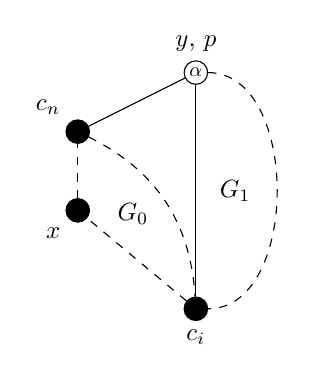
\begin{tikzpicture}[
		scale=1,
		every node/.style={circle, draw, minimum size=1mm, scale=0.9},
		every label/.append style={rectangle}
	]
  \node (c_n) [label=above left:$c_n$, fill] at (-1.5cm, 1.25cm) {};
  \node (p) [label=above:{$y$, $p$}] at (0cm, 2cm) {};
  \node (p_label) [draw=none, scale=0.8] at (0cm, 2cm) {$\alpha$};
  \node (x) [label=below left:$x$, fill] at (-1.5cm, 0.25cm) {};
  \node (c_i) [label=below:$c_i$, fill] at (0cm, -1cm) {};
  \node (G_0) [draw=none, ] at (-0.8cm, 0.2cm) {$G_0$};
  \node (G_1) [draw=none] at (0.5cm, 0.5cm) {$G_1$};
  \node (null) [draw=none] at (270:1.5cm) {};
  \draw (c_i) edge (x) [dashed];
  \draw (x) edge (c_n) [dashed];
  \draw (c_n) edge [bend left] (c_i) [dashed];
  \draw (c_n) edge (p);
  \draw (p) edge (c_i);
  \draw (p) edge [bend left=90] (c_i) [dashed];
\end{tikzpicture}
$\quad$
\begin{tikzpicture}[
		scale=1,
		every node/.style={circle, draw, minimum size=1mm, scale=0.9},
		every label/.append style={rectangle}
	]
  \node (null) [draw=none] at (0cm, 0.5cm) {$\rightarrow$};
  \node (null) [draw=none] at (270:1.5cm) {};
\end{tikzpicture}
$\quad$
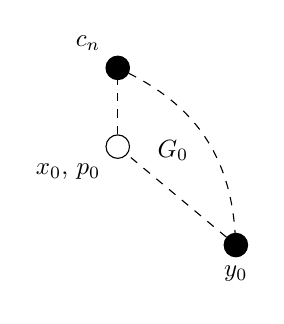
\begin{tikzpicture}[
		scale=1,
		every node/.style={circle, draw, minimum size=1mm, scale=0.9},
		every label/.append style={rectangle}
	]
  \node (c_n) [label=above left:$c_n$, fill] at (-1.5cm, 1.25cm) {};
  \node (x) [label=below left:{$x_0$, $p_0$}] at (-1.5cm, 0.25cm) {};
  \node (c_i) [label=below:$y_0$, fill] at (0cm, -1cm) {};
  \node (G_0) [draw=none, ] at (-0.8cm, 0.2cm) {$G_0$};
  \node (null) [draw=none] at (270:1.5cm) {};
  \draw (c_i) edge (x) [dashed];
  \draw (x) edge (c_n) [dashed];
  \draw (c_n) edge [bend left] (c_i) [dashed];
\end{tikzpicture}
$\quad$
\begin{tikzpicture}[
		scale=1,
		every node/.style={circle, draw, minimum size=1mm, scale=0.9},
		every label/.append style={rectangle}
	]
  \node (null) [draw=none] at (0cm, 0.5cm) {$\rightarrow$};
  \node (null) [draw=none] at (270:1.5cm) {};
\end{tikzpicture}
$\quad$
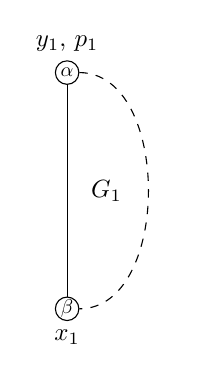
\begin{tikzpicture}[
		scale=1,
		every node/.style={circle, draw, minimum size=1mm, scale=0.9},
		every label/.append style={rectangle}
	]
  \node (p) [label=above:{$y_1$, $p_1$}] at (0cm, 2cm) {};
  \node (p_label) [draw=none, scale=0.8] at (0cm, 2cm) {$\alpha$};
  \node (c_i) [label=below:$x_1$] at (0cm, -1cm) {};
  \node (c_i_label) [draw=none, scale=0.8] at (0cm, -1cm) {$\beta$};
  \node (G_1) [draw=none] at (0.5cm, 0.5cm) {$G_1$};
  \node (null) [draw=none] at (270:1.5cm) {};
  \draw (p) edge (c_i);
  \draw (p) edge [bend left=90] (c_i) [dashed];
\end{tikzpicture}
\hfill\\
\textbf{Figure 3.5} The case $y=p$, $x\ne p$, and $c_i\not\in C[x,p)$.
\end{center}

\noindent Suppose $y=p$, $x\ne p$, and $c_i\not\in C[x,p)$. Color $x$ from $L_0(x)$ and apply the inductive
hypothesis to choose
$G_0$ from $L_0$ with $x_0=p_0=x$ and $y_0=c_i$. If $G_1$ exists we apply the inductive hypothesis again to
choose $G_1$ from $L$ with $x_1=c_i$, $y_1=y$, and $p_1=p$. Notice $c_i$ recieves at most one same color
neighbor in each $G_0$ and $G_1$. 

\begin{center}
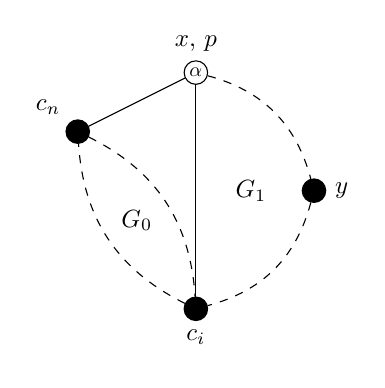
\begin{tikzpicture}[
		scale=1,
		every node/.style={circle, draw, minimum size=1mm, scale=0.9},
		every label/.append style={rectangle}
	]
  \node (c_n) [label=above left:$c_n$, fill] at (-1.5cm, 1.25cm) {};
  \node (p) [label=above:{$x$, $p$}] at (0cm, 2cm) {};
  \node (p_label) [draw=none, scale=0.8] at (0cm, 2cm) {$\alpha$};
  \node (y) [label=right:$y$, fill] at (1.5cm, 0.5cm) {};
  \node (c_i) [label=below:$c_i$, fill] at (0cm, -1cm) {};
  \node (G_0) [draw=none, ] at (-0.75cm, 0.12cm) {$G_0$};
  \node (G_1) [draw=none] at (0.7cm, 0.5cm) {$G_1$};
  \node (null) [draw=none] at (270:1.5cm) {};
  \draw (c_i) edge [bend left] (c_n) [dashed];
  \draw (c_n) edge [bend left] (c_i) [dashed];
  \draw (c_n) edge (p);
  \draw (p) edge (c_i);
  \draw (p) edge [bend left] (y) [dashed];
  \draw (y) edge [bend left] (c_i) [dashed];
\end{tikzpicture}
$\quad$
\begin{tikzpicture}[
		scale=1,
		every node/.style={circle, draw, minimum size=1mm, scale=0.9},
		every label/.append style={rectangle}
	]
  \node (null) [draw=none] at (0cm, 0.5cm) {$\rightarrow$};
  \node (null) [draw=none] at (270:1.5cm) {};
\end{tikzpicture}
$\quad$
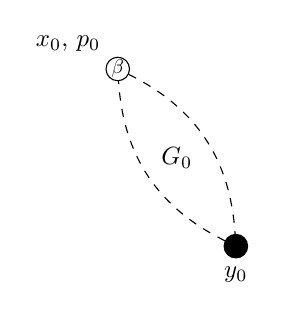
\begin{tikzpicture}[
		scale=1,
		every node/.style={circle, draw, minimum size=1mm, scale=0.9},
		every label/.append style={rectangle}
	]
  \node (c_n) [label=above left:{$x_0$, $p_0$}] at (-1.5cm, 1.25cm) {};
  \node (c_n_label) [draw=none, scale=0.8] at (-1.5cm, 1.25cm) {$\beta$};
  \node (c_i) [label=below:{$y_0$}, fill] at (0cm, -1cm) {};
  \node (G_0) [draw=none] at (-0.75cm, 0.12cm) {$G_0$};
  \node (null) [draw=none] at (270:1.5cm) {};
  \draw (c_i) edge [bend left] (c_n) [dashed];
  \draw (c_n) edge [bend left] (c_i) [dashed];
\end{tikzpicture}
$\quad$
\begin{tikzpicture}[
		scale=1,
		every node/.style={circle, draw, minimum size=1mm, scale=0.9},
		every label/.append style={rectangle}
	]
  \node (null) [draw=none] at (0cm, 0.5cm) {$\rightarrow$};
  \node (null) [draw=none] at (270:1.5cm) {};
\end{tikzpicture}
$\quad$
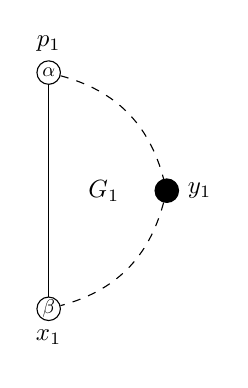
\begin{tikzpicture}[
		scale=1,
		every node/.style={circle, draw, minimum size=1mm, scale=0.9},
		every label/.append style={rectangle}
	]
  \node (p) [label=above:$p_1$] at (0cm, 2cm) {};
  \node (p_label) [draw=none, scale=0.8] at (0cm, 2cm) {$\alpha$};
  \node (y) [label=right:$y_1$, fill] at (1.5cm, 0.5cm) {};
  \node (c_i) [label=below:$x_1$] at (0cm, -1cm) {};
  \node (c_i_label) [draw=none, scale=0.8] at (0cm, -1cm) {$\beta$};
  \node (G_1) [draw=none] at (0.7cm, 0.5cm) {$G_1$};
  \node (null) [draw=none] at (270:1.5cm) {};
  \draw (p) edge (c_i);
  \draw (p) edge [bend left] (y) [dashed];
  \draw (y) edge [bend left] (c_i) [dashed];
\end{tikzpicture}
\hfill\\
\textbf{Figure 3.6} The case $x=p$, $y\ne p$, and $c_i\in C(y,x)$.
\end{center}

\noindent Suppose $x=p$, $y\ne p$, and $c_i\in C(y,x)$. Apply the
inductive hypothesis to choose $G_0$ from $L_0$ with $x_0=p_0=c_n$ and $y_0=c_i$. In this case $G_1$ must exist
and we apply the inductive
hypothesis to choose $G_1$ from $L$ with $x_1=c_i$, $y_1=y$, and $p_1=p$. Notice $c_i$ recieves at most one same
color neighbor in each $G_0$ and $G_1$.

\begin{center}
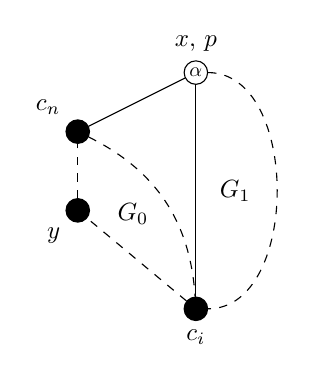
\begin{tikzpicture}[
		scale=1,
		every node/.style={circle, draw, minimum size=1mm, scale=0.9},
		every label/.append style={rectangle}
	]
  \node (c_n) [label=above left:$c_n$, fill] at (-1.5cm, 1.25cm) {};
  \node (p) [label=above:{$x$, $p$}] at (0cm, 2cm) {};
  \node (p_label) [draw=none, scale=0.8] at (0cm, 2cm) {$\alpha$};
  \node (y) [label=below left:$y$, fill] at (-1.5cm, 0.25cm) {};
  \node (c_i) [label=below:$c_i$, fill] at (0cm, -1cm) {};
  \node (G_0) [draw=none, ] at (-0.8cm, 0.2cm) {$G_0$};
  \node (G_1) [draw=none] at (0.5cm, 0.5cm) {$G_1$};
  \node (null) [draw=none] at (270:1.5cm) {};
  \draw (c_i) edge (y) [dashed];
  \draw (y) edge (c_n) [dashed];
  \draw (c_n) edge [bend left] (c_i) [dashed];
  \draw (c_n) edge (p);
  \draw (p) edge (c_i);
  \draw (p) edge [bend left=90] (c_i) [dashed];
\end{tikzpicture}
$\quad$
\begin{tikzpicture}[
		scale=1,
		every node/.style={circle, draw, minimum size=1mm, scale=0.9},
		every label/.append style={rectangle}
	]
  \node (null) [draw=none] at (0cm, 0.5cm) {$\rightarrow$};
  \node (null) [draw=none] at (270:1.5cm) {};
\end{tikzpicture}
$\quad$
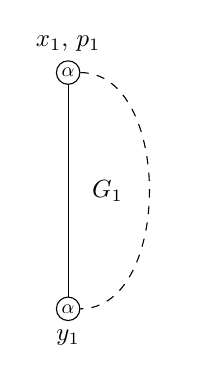
\begin{tikzpicture}[
		scale=1,
		every node/.style={circle, draw, minimum size=1mm, scale=0.9},
		every label/.append style={rectangle}
	]
  \node (p) [label=above:{$x_1$, $p_1$}] at (0cm, 2cm) {};
  \node (p_label) [draw=none, scale=0.8] at (0cm, 2cm) {$\alpha$};
  \node (c_i) [label=below:$y_1$] at (0cm, -1cm) {};
  \node (c_i_label) [draw=none, scale=0.8] at (0cm, -1cm) {$\alpha$};
  \node (G_1) [draw=none] at (0.5cm, 0.5cm) {$G_1$};
  \node (null) [draw=none] at (270:1.5cm) {};
  \draw (p) edge (c_i);
  \draw (p) edge [bend left=90] (c_i) [dashed];
\end{tikzpicture}
$\quad$
\begin{tikzpicture}[
		scale=1,
		every node/.style={circle, draw, minimum size=1mm, scale=0.9},
		every label/.append style={rectangle}
	]
  \node (null) [draw=none] at (0cm, 0.5cm) {$\rightarrow$};
  \node (null) [draw=none] at (270:1.5cm) {};
\end{tikzpicture}
$\quad$
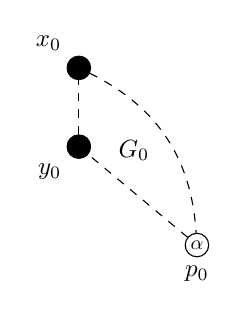
\begin{tikzpicture}[
		scale=1,
		every node/.style={circle, draw, minimum size=1mm, scale=0.9},
		every label/.append style={rectangle}
	]
  \node (c_n) [label=above left:$x_0$, fill] at (-1.5cm, 1.25cm) {};
  \node (y) [label=below left:$y_0$, fill] at (-1.5cm, 0.25cm) {};
  \node (c_i) [label=below:$p_0$] at (0cm, -1cm) {};
  \node (c_i_label) [draw=none, scale=0.8] at (0cm, -1cm) {$\alpha$};
  \node (G_0) [draw=none, ] at (-0.8cm, 0.2cm) {$G_0$};
  \node (null) [draw=none] at (270:1.5cm) {};
  \draw (c_i) edge (y) [dashed];
  \draw (y) edge (c_n) [dashed];
  \draw (c_n) edge [bend left] (c_i) [dashed];
\end{tikzpicture}
\hfill\\
\textbf{Figure 3.7} The case $x=p$, $y\ne p$, and $c_i\not\in C(y,x)$ (shown is the case $y\ne c_i$ and
$\alpha\in L(c_i)$).
\end{center}

\noindent Suppose $x=p$, $y\ne p$, and $c_i\not\in C(y,x)$. If
$\alpha\in L(c_i)$ we set $p_0=c_i$ and color $c_i$ with $\alpha$. Otherwise, set $p_0=c_n$ and color it with
the first color in $L_0(c_n)$, note $|L_0(c_i)|\ge 2$ in this case. Apply the inductive hypothesis to
choose $G_0$ from $L_0$ with $x_0=c_n$, $y_0=y$, and $p_0$. If $G_1$ exists, apply the inductive
hypothesis to choose $G_1$ from $L$ with $x_1=p_1=p$ and $y_1=c_i$. Notice if $p_0=c_i$, $c_i$ recieves at most
one same color neighbor in $G_0$ and the single same color neighbor $p$ in $G_1$. Furthermore, $p$ will recieve no
same color neighbor in $G_1$ other than $c_i$. If $p_0\ne c_i$, then $y_1=c_i$ is immediatley prior to
$p_1=p$ and $\alpha\not\in L(c_i)$. Thus $c_i$ will recieve no same color neighbors in $G_1$.

\begin{center}
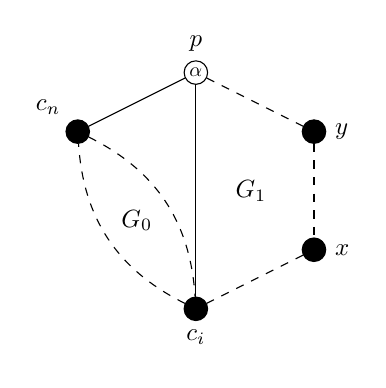
\begin{tikzpicture}[
		scale=1,
		every node/.style={circle, draw, minimum size=1mm, scale=0.9},
		every label/.append style={rectangle}
	]
  \node (c_n) [label=above left:$c_n$, fill] at (-1.5cm, 1.25cm) {};
  \node (p) [label=above:{$p$}] at (0cm, 2cm) {};
  \node (p_label) [draw=none, scale=0.8] at (0cm, 2cm) {$\alpha$};
  \node (y) [label=right:$y$, fill] at (1.5cm, 1.25cm) {};
  \node (x) [label=right:$x$, fill] at (1.5cm, -0.25cm) {};
  \node (c_i) [label=below:$c_i$, fill] at (0cm, -1cm) {};
  \node (G_0) [draw=none, ] at (-0.75cm, 0.12cm) {$G_0$};
  \node (G_1) [draw=none] at (0.7cm, 0.5cm) {$G_1$};
  \node (null) [draw=none] at (270:1.5cm) {};
  \draw (c_i) edge [bend left] (c_n) [dashed];
  \draw (c_n) edge [bend left] (c_i) [dashed];
  \draw (c_n) edge (p);
  \draw (p) edge (c_i);
  \draw (p) edge (y) [dashed];
  \draw (y) edge (x) [dashed];
  \draw (x) edge (c_i) [dashed];
\end{tikzpicture}
$\quad$
\begin{tikzpicture}[
		scale=1,
		every node/.style={circle, draw, minimum size=1mm, scale=0.9},
		every label/.append style={rectangle}
	]
  \node (null) [draw=none] at (0cm, 0.5cm) {$\rightarrow$};
  \node (null) [draw=none] at (270:1.5cm) {};
\end{tikzpicture}
$\quad$
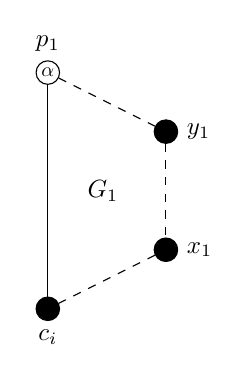
\begin{tikzpicture}[
		scale=1,
		every node/.style={circle, draw, minimum size=1mm, scale=0.9},
		every label/.append style={rectangle}
	]
  \node (p) [label=above:{$p_1$}] at (0cm, 2cm) {};
  \node (p_label) [draw=none, scale=0.8] at (0cm, 2cm) {$\alpha$};
  \node (y) [label=right:$y_1$, fill] at (1.5cm, 1.25cm) {};
  \node (x) [label=right:$x_1$, fill] at (1.5cm, -0.25cm) {};
  \node (c_i) [label=below:$c_i$, fill] at (0cm, -1cm) {};
  \node (G_1) [draw=none] at (0.7cm, 0.5cm) {$G_1$};
  \node (null) [draw=none] at (270:1.5cm) {};
  \draw (p) edge (c_i);
  \draw (p) edge (y) [dashed];
  \draw (y) edge (x) [dashed];
  \draw (x) edge (c_i) [dashed];
\end{tikzpicture}
$\quad$
\begin{tikzpicture}[
		scale=1,
		every node/.style={circle, draw, minimum size=1mm, scale=0.9},
		every label/.append style={rectangle}
	]
  \node (null) [draw=none] at (0cm, 0.5cm) {$\rightarrow$};
  \node (null) [draw=none] at (270:1.5cm) {};
\end{tikzpicture}
$\quad$
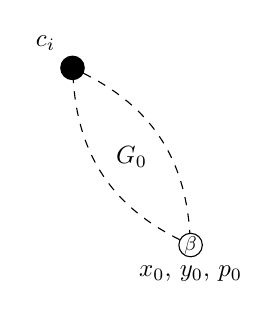
\begin{tikzpicture}[
		scale=1,
		every node/.style={circle, draw, minimum size=1mm, scale=0.9},
		every label/.append style={rectangle}
	]
  \node (c_n) [label=above left:$c_i$, fill] at (-1.5cm, 1.25cm) {};
  \node (c_i) [label=below:{$x_0$, $y_0$, $p_0$}] at (0cm, -1cm) {};
  \node (c_i_label) [draw=none, scale=0.8] at (0cm, -1cm) {$\beta$};
  \node (G_0) [draw=none, ] at (-0.75cm, 0.12cm) {$G_0$};
  \node (null) [draw=none] at (270:1.5cm) {};
  \draw (c_i) edge [bend left] (c_n) [dashed];
  \draw (c_n) edge [bend left] (c_i) [dashed];
\end{tikzpicture}
\hfill\\
\textbf{Figure 3.8} The case $x\ne p$, $y\ne p$, and $c_i\in C[x,p)$ (shown is the case $x\ne c_i$).
\end{center}

\noindent Suppose $x\ne p$, $y\ne p$, and $c_i\in C[x,p)$. In this case $G_1$ must exist and we apply
the inductive hypothesis to choose $G_1$ from $L$ with $x_1=x$, $y_1=y$, and $p_1=p$.
Apply the inductive hypothesis again to choose $G_0$ from
$L_0$ with $x_0=y_0=p_0=c_i$. Note that $c_i$ was precolored from the choosing of $G_1$ and recieves
no same color neighbors in $G_0$ so the combined coloring forms a path choosing of $G$ from $L$.

\begin{center}
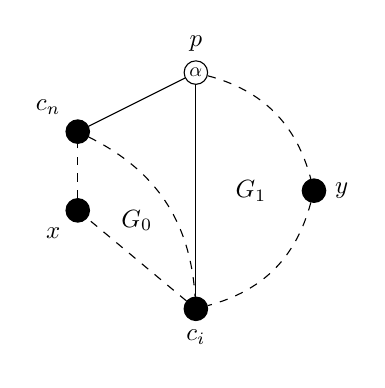
\begin{tikzpicture}[
		scale=1,
		every node/.style={circle, draw, minimum size=1mm, scale=0.9},
		every label/.append style={rectangle}
	]
  \node (c_n) [label=above left:$c_n$, fill] at (-1.5cm, 1.25cm) {};
  \node (p) [label=above:{$p$}] at (0cm, 2cm) {};
  \node (p_label) [draw=none, scale=0.8] at (0cm, 2cm) {$\alpha$};
  \node (x) [label=below left:$x$, fill] at (-1.5cm, 0.25cm) {};
  \node (y) [label=right:$y$, fill] at (1.5cm, 0.5cm) {};
  \node (c_i) [label=below:$c_i$, fill] at (0cm, -1cm) {};
  \node (G_0) [draw=none, ] at (-0.75cm, 0.12cm) {$G_0$};
  \node (G_1) [draw=none] at (0.7cm, 0.5cm) {$G_1$};
  \node (null) [draw=none] at (270:1.5cm) {};
  \draw (c_i) edge (x) [dashed];
  \draw (x) edge (c_n) [dashed];
  \draw (c_n) edge [bend left] (c_i) [dashed];
  \draw (c_n) edge (p);
  \draw (p) edge (c_i);
  \draw (p) edge [bend left] (y) [dashed];
  \draw (y) edge [bend left] (c_i) [dashed];
\end{tikzpicture}
$\quad$
\begin{tikzpicture}[
		scale=1,
		every node/.style={circle, draw, minimum size=1mm, scale=0.9},
		every label/.append style={rectangle}
	]
  \node (null) [draw=none] at (0cm, 0.5cm) {$\rightarrow$};
  \node (null) [draw=none] at (270:1.5cm) {};
\end{tikzpicture}
$\quad$
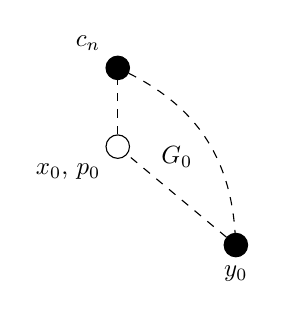
\begin{tikzpicture}[
		scale=1,
		every node/.style={circle, draw, minimum size=1mm, scale=0.9},
		every label/.append style={rectangle}
	]
  \node (c_n) [label=above left:{$c_n$}, fill] at (-1.5cm, 1.25cm) {};
  \node (x) [label=below left:{$x_0$, $p_0$}] at (-1.5cm, 0.25cm) {};
  \node (c_i) [label=below:{$y_0$}, fill] at (0cm, -1cm) {};
  \node (G_0) [draw=none] at (-0.75cm, 0.12cm) {$G_0$};
  \node (null) [draw=none] at (270:1.5cm) {};
  \draw (c_i) edge (x) [dashed];
  \draw (x) edge (c_n) [dashed];
  \draw (c_n) edge [bend left] (c_i) [dashed];
\end{tikzpicture}
$\quad$
\begin{tikzpicture}[
		scale=1,
		every node/.style={circle, draw, minimum size=1mm, scale=0.9},
		every label/.append style={rectangle}
	]
  \node (null) [draw=none] at (0cm, 0.5cm) {$\rightarrow$};
  \node (null) [draw=none] at (270:1.5cm) {};
\end{tikzpicture}
$\quad$
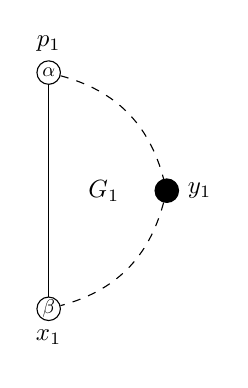
\begin{tikzpicture}[
		scale=1,
		every node/.style={circle, draw, minimum size=1mm, scale=0.9},
		every label/.append style={rectangle}
	]
  \node (p) [label=above:$p_1$] at (0cm, 2cm) {};
  \node (p_label) [draw=none, scale=0.8] at (0cm, 2cm) {$\alpha$};
  \node (y) [label=right:$y_1$, fill] at (1.5cm, 0.5cm) {};
  \node (c_i) [label=below:$x_1$] at (0cm, -1cm) {};
  \node (c_i_label) [draw=none, scale=0.8] at (0cm, -1cm) {$\beta$};
  \node (G_1) [draw=none] at (0.7cm, 0.5cm) {$G_1$};
  \node (null) [draw=none] at (270:1.5cm) {};
  \draw (p) edge (c_i);
  \draw (p) edge [bend left] (y) [dashed];
  \draw (y) edge [bend left] (c_i) [dashed];
\end{tikzpicture}
\hfill\\
\textbf{Figure 3.9} The case $x\ne p$, $y\ne p$, and $c_i\in C(y,x)$.
\end{center}

\noindent Suppose $x\ne p$, $y\ne p$, and $c_i\in C(y,x)$. Apply
the inductive hypothesis to choose $G_0$ from $L_0$ with $x_0=p_0=x$ and $y_0=c_i$. In this case $G_1$ must exist
and we apply the inductive
hypothesis again to choose $G_1$ from $L$ with $x_1=c_i$, $y_1=y$, and $p_1=p$. Notice $c_i$ recieves at most
one same color neighbor in each $G_0$ and $G_1$.

\begin{center}
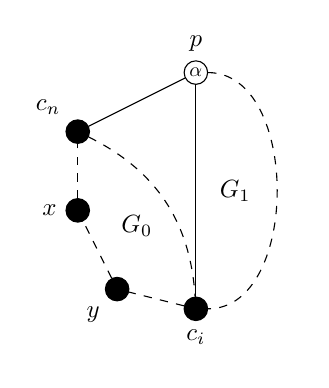
\begin{tikzpicture}[
		scale=1,
		every node/.style={circle, draw, minimum size=1mm, scale=0.9},
		every label/.append style={rectangle}
	]
  \node (c_n) [label=above left:$c_n$, fill] at (-1.5cm, 1.25cm) {};
  \node (p) [label=above:{$p$}] at (0cm, 2cm) {};
  \node (p_label) [draw=none, scale=0.8] at (0cm, 2cm) {$\alpha$};
  \node (x) [label=left:$x$, fill] at (-1.5cm, 0.25cm) {};
  \node (y) [label=below left:$y$, fill] at (-1cm, -0.75cm) {};
  \node (c_i) [label=below:$c_i$, fill] at (0cm, -1cm) {};
  \node (G_0) [draw=none, ] at (-0.75cm, 0.05cm) {$G_0$};
  \node (G_1) [draw=none] at (0.5cm, 0.5cm) {$G_1$};
  \node (null) [draw=none] at (270:1.5cm) {};
  \draw (c_i) edge (y) [dashed];
  \draw (y) edge (x) [dashed];
  \draw (x) edge (c_n) [dashed];
  \draw (c_n) edge [bend left] (c_i) [dashed];
  \draw (c_n) edge (p);
  \draw (p) edge (c_i);
  \draw (p) edge [bend left=90] (c_i) [dashed];
\end{tikzpicture}
$\quad$
\begin{tikzpicture}[
		scale=1,
		every node/.style={circle, draw, minimum size=1mm, scale=0.9},
		every label/.append style={rectangle}
	]
  \node (null) [draw=none] at (0cm, 0.5cm) {$\rightarrow$};
  \node (null) [draw=none] at (270:1.5cm) {};
\end{tikzpicture}
$\quad$
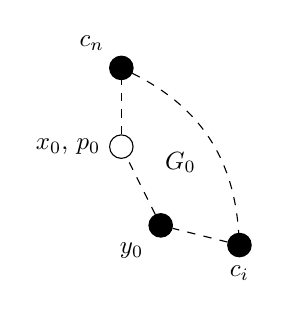
\begin{tikzpicture}[
		scale=1,
		every node/.style={circle, draw, minimum size=1mm, scale=0.9},
		every label/.append style={rectangle}
	]
  \node (c_n) [label=above left:{$c_n$}, fill] at (-1.5cm, 1.25cm) {};
  \node (x) [label=left:{$x_0$, $p_0$}] at (-1.5cm, 0.25cm) {};
  \node (y) [label=below left:$y_0$, fill] at (-1cm, -0.75cm) {};
  \node (c_i) [label=below:$c_i$, fill] at (0cm, -1cm) {};
  \node (G_0) [draw=none, ] at (-0.75cm, 0.05cm) {$G_0$};
  \node (null) [draw=none] at (270:1.5cm) {};
  \draw (c_i) edge (y) [dashed];
  \draw (y) edge (x) [dashed];
  \draw (x) edge (c_n) [dashed];
  \draw (c_n) edge [bend left] (c_i) [dashed];
\end{tikzpicture}
$\quad$
\begin{tikzpicture}[
		scale=1,
		every node/.style={circle, draw, minimum size=1mm, scale=0.9},
		every label/.append style={rectangle}
	]
  \node (null) [draw=none] at (0cm, 0.5cm) {$\rightarrow$};
  \node (null) [draw=none] at (270:1.5cm) {};
\end{tikzpicture}
$\quad$
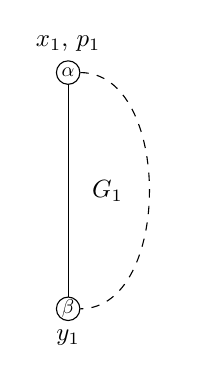
\begin{tikzpicture}[
		scale=1,
		every node/.style={circle, draw, minimum size=1mm, scale=0.9},
		every label/.append style={rectangle}
	]
  \node (p) [label=above:{$x_1$, $p_1$}] at (0cm, 2cm) {};
  \node (p_label) [draw=none, scale=0.8] at (0cm, 2cm) {$\alpha$};
  \node (c_i) [label=below:$y_1$] at (0cm, -1cm) {};
  \node (c_i_label) [draw=none, scale=0.8] at (0cm, -1cm) {$\beta$};
  \node (G_1) [draw=none] at (0.5cm, 0.5cm) {$G_1$};
  \node (null) [draw=none] at (270:1.5cm) {};
  \draw (p) edge (c_i);
  \draw (p) edge [bend left=90] (c_i) [dashed];
\end{tikzpicture}
\hfill\\
\textbf{Figure 3.10} The case $x\ne p$, $y\ne p$, and $c_i\in C(p,y]$ (shown is the case $y\ne c_i$ and
$\alpha\not\in L(c_i)$).
\end{center}

\noindent Finally, suppose $x\ne p$, $y\ne p$, and $c_i\in C(p,y]$. If
$\alpha\in L(c_i)$ we set $p_0=c_i$ and color $c_i$ with $\alpha$. Otherwise, define $p_0=c_1$ and color it from
$L_0(c_1)$, noting $|L_0(c_i)|\ge 2$ in this case. Apply the inductive hypothesis to
choose $G_0$ from $L_0$ with $x_0=x$, $y_0=y$, and $p_0$. If $G_1$ exists, apply the inductive again
hypothesis to choose $G_1$ from $L$ with $x_1=p_1=p$ and $y_1=c_i$. Note that $c_i$ was precolored by our
choosing of $G_0$. If $p_0=c_i$, $c_i$ recieves at most one same
color neighbor in $G_0$ and the single same color neighbor $p$ in $G_1$. Furthermore, $p$ will recieve no
same color neighbor in $G_1$ other than $c_i$. If $p_0\ne c_i$, then $y_1=c_i$ is immediatley prior to
$p_1=p$ and $\alpha\not\in L(c_i)$. Thus $c_i$ will recieve no same color neighbors in $G_1$.\\
\end{proof}

\begin{adjustwidth}{1.5em}{1.5em}
\noindent\textbf{Corollary 4.} All planar graphs are path $3$-choosable.\\
\end{adjustwidth}

\begin{proof}
Let $G$ be a plane graph and $L$ an assignment of size $3$ color lists to each vertex of $G$. As adding edges does
not make $G$ easier to color, augment $G$ with edges until it is triangulated (maximally planar).
Assign $x$ and $y$ to be distinct vertices on the outer face. Color $x$ from $L(x)$
and assign $p=x$. Apply Theorem 3 to path choose $G$ from $L$ accordingly.\\
\end{proof}

\subsection*{Path 3-Choosing Algorithm}

\noindent Let $G$ be a weakly triangulated plane graph with vertices $x$, $y$, and $p$ defined and
colored in accordance with Theorem 3. We will again denote the outer face of $G$ as
$C=c_0c_1\ldots c_n$ with $c_0=p$.
We will denote the embedding ordered $N(p)$ as $n_0\ldots n_k$, with $n_0=c_1$ and
$n_k=c_n$. We will denote the parameters for an application of the algorithm as the tuple $(G, x, y, p)$.
The path $3$-choosing algorithm proceeds as follows:

\begin{enumerate}
\item If $p$ has not been colored, color $p$ from $L(p)$;
\item If $n_k=y$ and $\alpha\in L(y)$, color $y$ with $\alpha$ and apply the algorithm to $G$ with $x'=p'=y$ and
$y'=p$;
\item Remove $\alpha$ from $L(n_k)$;
\item For $j=k-1$ to $0$: if $n_j\in C$ terminate, otherwise remove $\alpha$ from $L(n_j)$;
\item If $c_i\not\in C(p,y]$ remove $\alpha$ from $L(c_i)$;
\item We now have $n_j=c_i\in C$ and define $G_0$ as the subgraph with outer face
$C_0=c_i\ldots c_nn_{k-1}\ldots n_{j-1}$ and $G_1$ as the subgraph with outer face $c_0\ldots c_i$. If $c_i=c_1$
we ignore $G_1$;
\begin{enumerate}
\item If $x=y=p$, apply the algorithm first to $(G_0, c_n, c_i, c_n)$ and then to $(G_1, c_i, p, p)$;
\item If $y=p$, $x\ne p$, and $c_i\in C[x,p)$, apply the algorithm first to $(G_1, x, p, p)$ and then
$(G_0, c_i, c_i, c_i)$;
\item If $y=p$, $x\ne p$, and $c_i\in C(y,x)$, apply the algorithm first to $(G_0, x, c_i, x)$ and then to $(G_1, c_i, p, p)$;
\item If $x=p$, $y\ne p$, and $c_i\in C(y,x)$, apply the algorithm first to $(G_0, c_n, c_i, c_n)$ and then to $(G_1, c_i, p, y)$;
\item If $x=p$, $y\ne p$, $c_i\in C(p,y]$, and $\alpha\in L(c_i)$, color $c_i$ with $\alpha$ and apply the
algorithm first to $(G_1, p, c_i, p)$ and then to $(G_0, c_n, y, c_i)$;
\item If $x=p$, $y\ne p$, $c_i\in C(p,y]$, and $\alpha\not\in L(c_i)$, apply the
algorithm first to $(G_1, p, c_i, p)$ and then to $(G_0, c_n, y, c_n)$;
\item If $x\ne p$, $y\ne p$, $c_i\in C[x,p)$, apply the algorithm first to $(G_1, x, p, y)$ and then to
$(G_0, c_i, c_i, c_i)$;
\item If $x\ne p$, $y\ne p$, $c_i\in C(y,x)$, apply the algorithm first to $(G_0, x, c_i, x)$ and then to
$(G_1, c_i, y, p)$;
\item If $x\ne p$, $y\ne p$, $c_i\in C(p,y]$, and $\alpha\in L(c_i)$, color $c_i$ with $\alpha$ and apply the
algorithm first to $(G_0, x, y, c_i)$ and then to $(G_1, p, c_i, p)$;
\item If $x\ne p$, $y\ne p$, $c_i\in C(p,y]$, and $\alpha\not\in L(c_i)$, apply the
algorithm first to $(G_0, x, y, x)$ and then to $(G_1, p, c_i, p)$.
\end{enumerate}
\end{enumerate}

\subsection*{Implementing the Path 3-Choosing Algorithm}

Let $G$ be a $2$-connected weakly triangulated plane graph represented as an incidence list (or adjacency list)
and an ordering of edges around each vertex following a planar embedding.
We will track subgraphs by marking each vertex with a \emph{state} of \emph{interior},
\emph{face}, or \emph{colored}. Vertices will only change in state from \emph{interior} to \emph{face} to
\emph{colored}. Each \emph{face} and \emph{colored} vertex will have a \emph{neighbor range}
that tracks the range of edges in its ordered incidence list that belong to the current subgraph. This range
will start with the next vertex on the outer face and end with the previous.
Therefore we may walk clockwise along the outer face from a
\emph{face} vertex $v$ simply by proceeding to the first vertex in its \emph{neighbor range}.\\

\noindent To be able to perform the path $3$-choosing algorithm above we must also determine where each
\emph{face} vertex lies on the outer face with respect to $x$, $y$, and $p$. Each vertex will recieve a mark
associating it with a face segment. We will denote $C[x,p)$ as $s_p$, $C(p,y]$ as $s_y$, and $C(y,x)$ as $s_x$.
Each face segment may simply be represented by an integer type. The face
segments $s_p$ and $s_y$ will need to be joined in the case $\alpha\not\in L(c_i)$
and $c_i\in C(p,y]$ since $p$ will be moved away to start a new path. We utilize a disjoint set data structure,
as described in [u], to allow efficient union and find operations on face segments.

\begin{center}
\begin{tikzpicture}[
		scale=1,
		every node/.style={circle, draw, minimum size=1mm, scale=0.9},
		every label/.append style={rectangle}
	]
  \node (p) [label=above:{$p$}, fill] at (90:1cm) {};
  \node (x) [label=below left:{$x$}, fill] at (210:1cm) {};
  \node (y) [label=below right:{$y$}, fill] at (330:1cm) {};
  \node (sp) [draw=none] at (150:1.25cm) {$s_p$};
  \node (sy) [draw=none] at (30:1.25cm) {$s_y$};
  \node (sy) [draw=none] at (270:1.25cm) {$s_x$};
  \node (null) [draw=none] at (270:1.5cm) {};
  \draw (p) edge [bend left] (y) [dashed];
  \draw (y) edge [bend left] (x) [dashed];
  \draw (x) edge [bend left] (p) [dashed];
\end{tikzpicture}
\hfill\\
\textbf{Figure 3.11} The face segments of $G$.
\end{center}

\noindent Some additional steps must be added to the path $3$-choosing algorithm to maintain each data structure
during its operation. In the case that we color $y$ and rename vertices in step (2) we must also rename face
segments to swap $s_x$ with $s_y$ (see figure 3.2). In step (4) we perform
the following for each $n_j$, not including $c_i$, in addition to the regular steps of the algorithm:

\begin{enumerate}
\item Initialize $n_j$'s \emph{neighbor range} and set its \emph{state} to \emph{face};
\item Set $n_j$'s \emph{face location} to $s_p$, creating $s_p$ if it doesn't exist;
\item Contract the \emph{neighbor range} of $n_j$ to remove $p$ from its incidence list.
\end{enumerate}

\noindent Once the above procedure terminates we will have located $c_i$. We have almost fully determined $G_0$
and $G_1$ by our tracking of \emph{state} and \emph{neighbor range}. It only remains to find
the \emph{neighbor range} for $c_i$ in both $G_0$ and $G_1$. This can be achieved by locating $p$ in
$c_i$'s incidence list and splitting the \emph{neighbor range} of $c_i$ at the $pc_i$ edge. Comparing $c_i$, $x$,
$y$, and $p$, along with the \emph{face location} and \emph{state} properties for each we may determine which case
to apply in step (6). In each recursive call we must also pass any face segments that appear and rename
each accordding to their position with respect to the new assignments of $x$, $y$, and $p$. As noted earlier,
in (6e) and (6j) for $G_0$ we set $s_y$ to be the union of $s_p$ and $s_y$ (see figure 3.10).

\subsection*{Time Complexity}

First note that $G$ is planar so $O(|E|)=O(|V|)$. When a vertex is assigned as $p$ we will iterate through
its incidence list at most once. This is due to the fact that when each neighbor $n_j$ is hit, we remove $p$ from $n_j$'s
\emph{neighbor range}. Once each neighbor has been hit, $p$ has been effectively removed from the graph.
Therefore step (4) iterates through each edge in $E(G)$ at most twice, once for each incident vertex. Furthermore,
steps (1) through (3) will occur at most once for each iteration of step (4). Thus this process has complexity
$O(|E|)=O(|V|)$.\\

\noindent We will be performing numerous unions and finds throughout the operation of the algorithm, but no more
than $O(|V|)$ by the same reasoning as above. The only unions that will be made are between $s_p$ and
$s_y$. We may also notice that the segment $s_p$ is always a singleton in our disjoint set structure, only created
when new \emph{interior} vertices are added to the outer face while removing $p$. Therefore the complexity of
each union and find operation is $O(1)$ and the complexity of maintaining our face segment 
disjoint set structure over the entire operation of the algorithm is $O(|V|)$.\\

\noindent The remaining expensive operation
is locating the edge $c_ip$ in $c_i$'s incidence list. If $c_ip$ is an edge on the outer face, $c_i=c_1$ and
this lookup is constant time using the tracked \emph{neighbor range}. Otherwise, $c_ip$ is not an edge in
the outer face. We perform a neighbor lookup to find the edge with complexity $O(|E|/|V|)$.
After this step $c_ip$ will be in the outer face of both $G_0$ and $G_1$. Therefore we perform at most one lookup
for each edge in $E(G)$. This gives a complexity of $O(|E||E|/|V|)=O(|V|)$.\\

\noindent Therefore the complexity of the path $3$-choosing algorithm is $O(|V|)$.

\begin{comment}
\begin{algorithm}
\LinesNumbered
\DontPrintSemicolon
\KwIn{Plane graph $G$ and paths $P=p_0\ldots p_n$ and $Q=q_0\ldots q_m$}
\Begin{
	\Repeat{$t_0\not\in P\cup Q$} {
		$t_0\longleftarrow$ vertex forming face with $p_0$ and $q_0$\;
		\If{$t_0 = p_1$} {
			$P\longleftarrow P - p_0$\;
		}
		\ElseIf{$t_0 = q_1$} {
			$Q\longleftarrow Q - q_0$\; 
		}
	}
	\Repeat{$t_1\not\in P\cup Q$} {
		$t_1\longleftarrow$ vertex forming face with $p_n$ and $q_m$\;
		\If{$t_1 = p_{n-1}$} {
			$P\longleftarrow P - p_n$\;
		}
		\ElseIf{$t_1 = q_{m-1}$} {
			$Q\longleftarrow Q - q_m$\; 
		}
	}
	perform BFS starting at $t_1$\;
	\If{BFS finds $t_0$} {
		$T\longleftarrow$ BFS path $t_0$ to $t_1$\;
	}
	\Else {
		we hit an vertex $u$ with neighbors $p_i\in P$ and $q_j\in Q$\;
		$T\longleftarrow$ BFS path $u$ to $t_1$\;
		recurse on subgraph bounded by $p_0\ldots p_i$ and $q_0\ldots q_j$\;
		$P\longleftarrow p_i\ldots p_n$\;
		$Q\longleftarrow q_j\ldots q_m$\;
	}
	recurse on subgraph bounded by $P$ and $T$\;
	recurse on subgraph bounded by $T$ and $Q$\;
}
\caption{Path 3-Color}
\end{algorithm}

\end{comment}

\section*{References}

\begin{tabularx}{\linewidth}{lX}
[1] & Hartman, C., "Extremal problems in graph theory," Ph.D. thesis, Department of Mathematics,
University of Illinois at Urbana-Champaign, 1997.\\\relax
[2] & Skrekovski, R., "List improper colourings of planar graphs,"
\emph{Combinatorics, Probability and Computing}, vol. 8, pp. 293-299, 1999.\\\relax
[3] & Eaton, N., N. Hull, "Defective list colorings of planar graphs,"
\emph{Bulletin of the Institute for Combinatorics and its Applications}, 1999.\\\relax
[4] & Poh, K., "On the linear vertex-arboricity of a planar graph," \emph{Journal of Graph Theory},
vol. 14, pp. 73-75, 1990\\\relax
[5] & Thomassen, C., "Every planar graph is 4-choosable," \emph{Journal of Combinatorial Theory},
Series B, 1994\\\relax

%[5] & Kant, G., "Algorithms for drawing planar graphs," Ph.D. thesis, Department of Computer Science,
%Utrecht University, 1993.\\\relax
%[6] & Tarjan, R., "Depth-first search and linear graph algorithms," SIAM Journal on Computing, vol. 1, pp.
%146-160, 1972.\\\relax
\end{tabularx}



\end{document}
